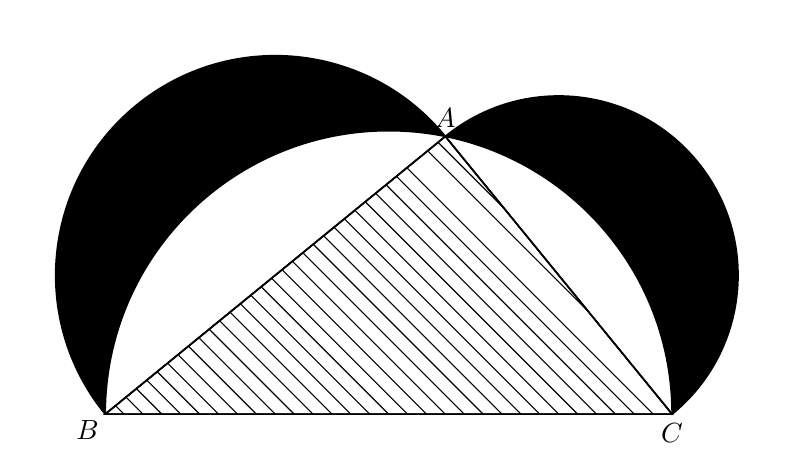
\begin{tikzpicture}[x=1.2cm,y=1.2cm,line width=.6pt,font=\normalsize]
\coordinate (B) at (0,0);
\coordinate (C) at (6,0);
\coordinate (A) at (3.6,2.9393876913);
% black lunes: AB semicircle (exterior) and AC semicircle (exterior, ccw via 489.23)
\fill[black] (B) -- (A) arc[start angle=39.2315204836,end angle=219.2315204836,radius=2.3237900077] -- cycle;
\fill[black] (A) -- (C) arc[start angle=309.2315204836,end angle=489.2315204836,radius=1.8973665961] -- cycle;
% white big semicircle with diameter BC (upper, contains triangle)
\fill[white] (B) -- (C) arc[start angle=0,end angle=180,radius=3] -- cycle;
% hatched triangle (region I): manually drawn diagonal hatch clipped to triangle
\draw[line width=.4pt] (0.2000000000,0.0000000000)--(0.1101020514,0.0898979486);
\draw[line width=.4pt] (0.4000000000,0.0000000000)--(0.2202041029,0.1797958971);
\draw[line width=.4pt] (0.6000000000,0.0000000000)--(0.3303061543,0.2696938457);
\draw[line width=.4pt] (0.8000000000,0.0000000000)--(0.4404082058,0.3595917942);
\draw[line width=.4pt] (1.0000000000,0.0000000000)--(0.5505102572,0.4494897428);
\draw[line width=.4pt] (1.2000000000,0.0000000000)--(0.6606123087,0.5393876913);
\draw[line width=.4pt] (1.4000000000,0.0000000000)--(0.7707143601,0.6292856399);
\draw[line width=.4pt] (1.6000000000,0.0000000000)--(0.8808164115,0.7191835885);
\draw[line width=.4pt] (1.8000000000,0.0000000000)--(0.9909184630,0.8090815370);
\draw[line width=.4pt] (2.0000000000,0.0000000000)--(1.1010205144,0.8989794856);
\draw[line width=.4pt] (2.2000000000,0.0000000000)--(1.2111225659,0.9888774341);
\draw[line width=.4pt] (2.4000000000,0.0000000000)--(1.3212246173,1.0787753827);
\draw[line width=.4pt] (2.6000000000,0.0000000000)--(1.4313266688,1.1686733312);
\draw[line width=.4pt] (2.8000000000,0.0000000000)--(1.5414287202,1.2585712798);
\draw[line width=.4pt] (3.0000000000,0.0000000000)--(1.6515307717,1.3484692283);
\draw[line width=.4pt] (3.2000000000,0.0000000000)--(1.7616328231,1.4383671769);
\draw[line width=.4pt] (3.4000000000,0.0000000000)--(1.8717348745,1.5282651255);
\draw[line width=.4pt] (3.6000000000,0.0000000000)--(1.9818369260,1.6181630740);
\draw[line width=.4pt] (3.8000000000,0.0000000000)--(2.0919389774,1.7080610226);
\draw[line width=.4pt] (4.0000000000,0.0000000000)--(2.2020410289,1.7979589711);
\draw[line width=.4pt] (4.2000000000,0.0000000000)--(2.3121430803,1.8878569197);
\draw[line width=.4pt] (4.4000000000,0.0000000000)--(2.4222451318,1.9777548682);
\draw[line width=.4pt] (4.6000000000,0.0000000000)--(2.5323471832,2.0676528168);
\draw[line width=.4pt] (4.8000000000,0.0000000000)--(2.6424492346,2.1575507654);
\draw[line width=.4pt] (5.0000000000,0.0000000000)--(2.7525512861,2.2474487139);
\draw[line width=.4pt] (5.2000000000,0.0000000000)--(2.8626533375,2.3373466625);
\draw[line width=.4pt] (5.4000000000,0.0000000000)--(2.9727553890,2.4272446110);
\draw[line width=.4pt] (5.6000000000,0.0000000000)--(3.0828574404,2.5171425596);
\draw[line width=.4pt] (5.8000000000,0.0000000000)--(3.1929594919,2.6070405081);
\draw[line width=.4pt] (5.1101020514,1.0898979486)--(3.4131635947,2.7868364053);
\draw[line width=.4pt] (4.2202041029,2.1797958971)--(3.5232656462,2.8767343538);
% outlines
\draw (B) -- (A) arc[start angle=39.2315204836,end angle=219.2315204836,radius=2.3237900077] -- cycle;
\draw (A) -- (C) arc[start angle=309.2315204836,end angle=489.2315204836,radius=1.8973665961] -- cycle;
\draw (B) -- (C) arc[start angle=0,end angle=180,radius=3] -- cycle;
\draw (A) -- (B) -- (C) -- cycle;
% labels in visible whitespace, clear of strokes
\node[below left=2pt,inner sep=0pt] at (B) {$B$};
\node[below=3pt,inner sep=0pt] at (C) {$C$};
\node[above=3pt,inner sep=0pt] at (A) {$A$};
\end{tikzpicture}
